\documentclass{article}
\usepackage{graphicx}
\usepackage{geometry}
 \geometry{a4paper,
  left=20mm,
  right=20mm,
  top=20mm,
 bottom=20mm,
 }
\usepackage{booktabs}
\usepackage{subcaption}
\usepackage{comment}
\usepackage{amsmath} %per sistemi eq

\begin{document}
\title{Numerical integration on the Lorenz system}
\author{Federico Giacobbe}
\date{October 2025}
\maketitle
This paper presents some key characteristics of chaotic systems, analyzing the results of some simulations of the Lorenz model.
\begin{equation}
    \begin{cases}
        \dot{x}= \sigma(y-x) \\
        \dot{y}= rx-xz-y \\
        \dot{z}=xy-bz
    \end{cases}
\end{equation}
\section{Numerical integration}
The system is integrated up to t=60 and with a time step dt = 0.005, using the forward Euler method and initial conditions $(x,y,z) = (9,10,18)$. Two integrations are performed with two different sets of parameters: Set A $\sigma,b,r=(10,8/3,28)$ and Set B $\sigma,b,r=(10,8/3,9)$.The graphs of the trajectories on the xz plane are discussed below.

\begin{figure}[htbp]
    \centering
    \begin{subfigure}[t]{0.49\textwidth}
        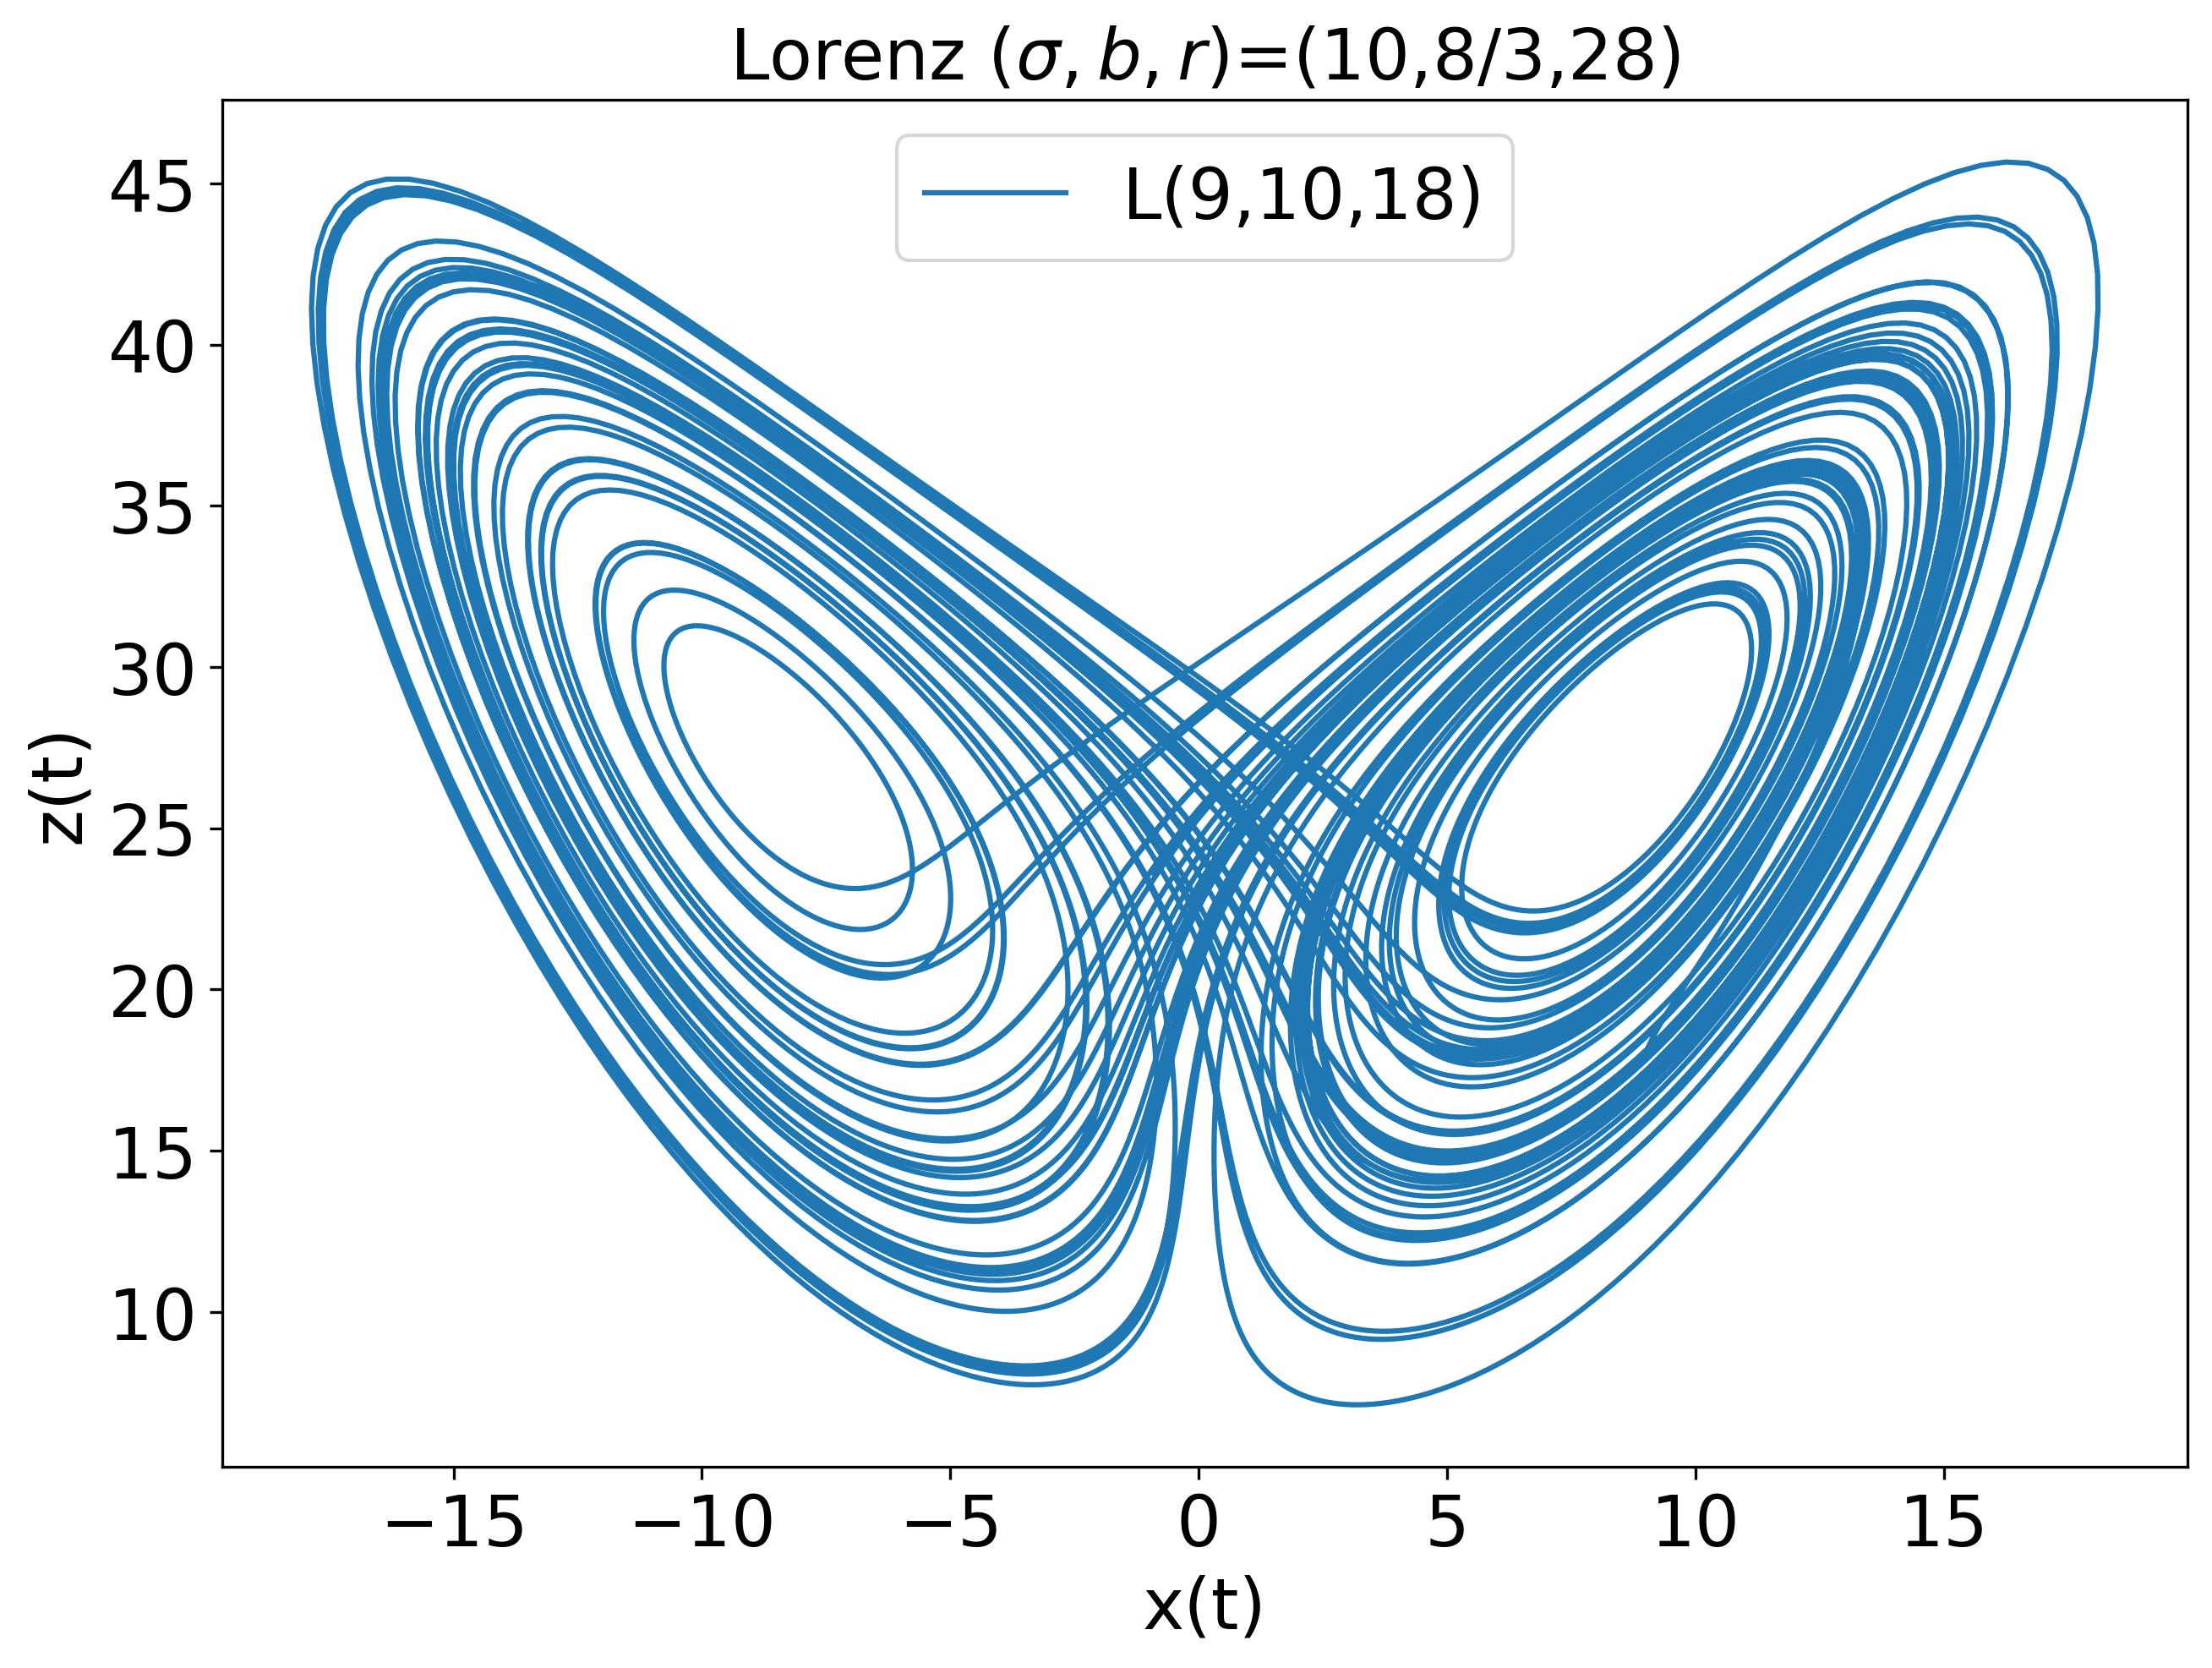
\includegraphics[width=\textwidth]{../xz_A.jpg}
        \caption{Set A}
        \label{fig:xz_a}
    \end{subfigure}
    \hfill
    \begin{subfigure}[t]{0.49\textwidth}
        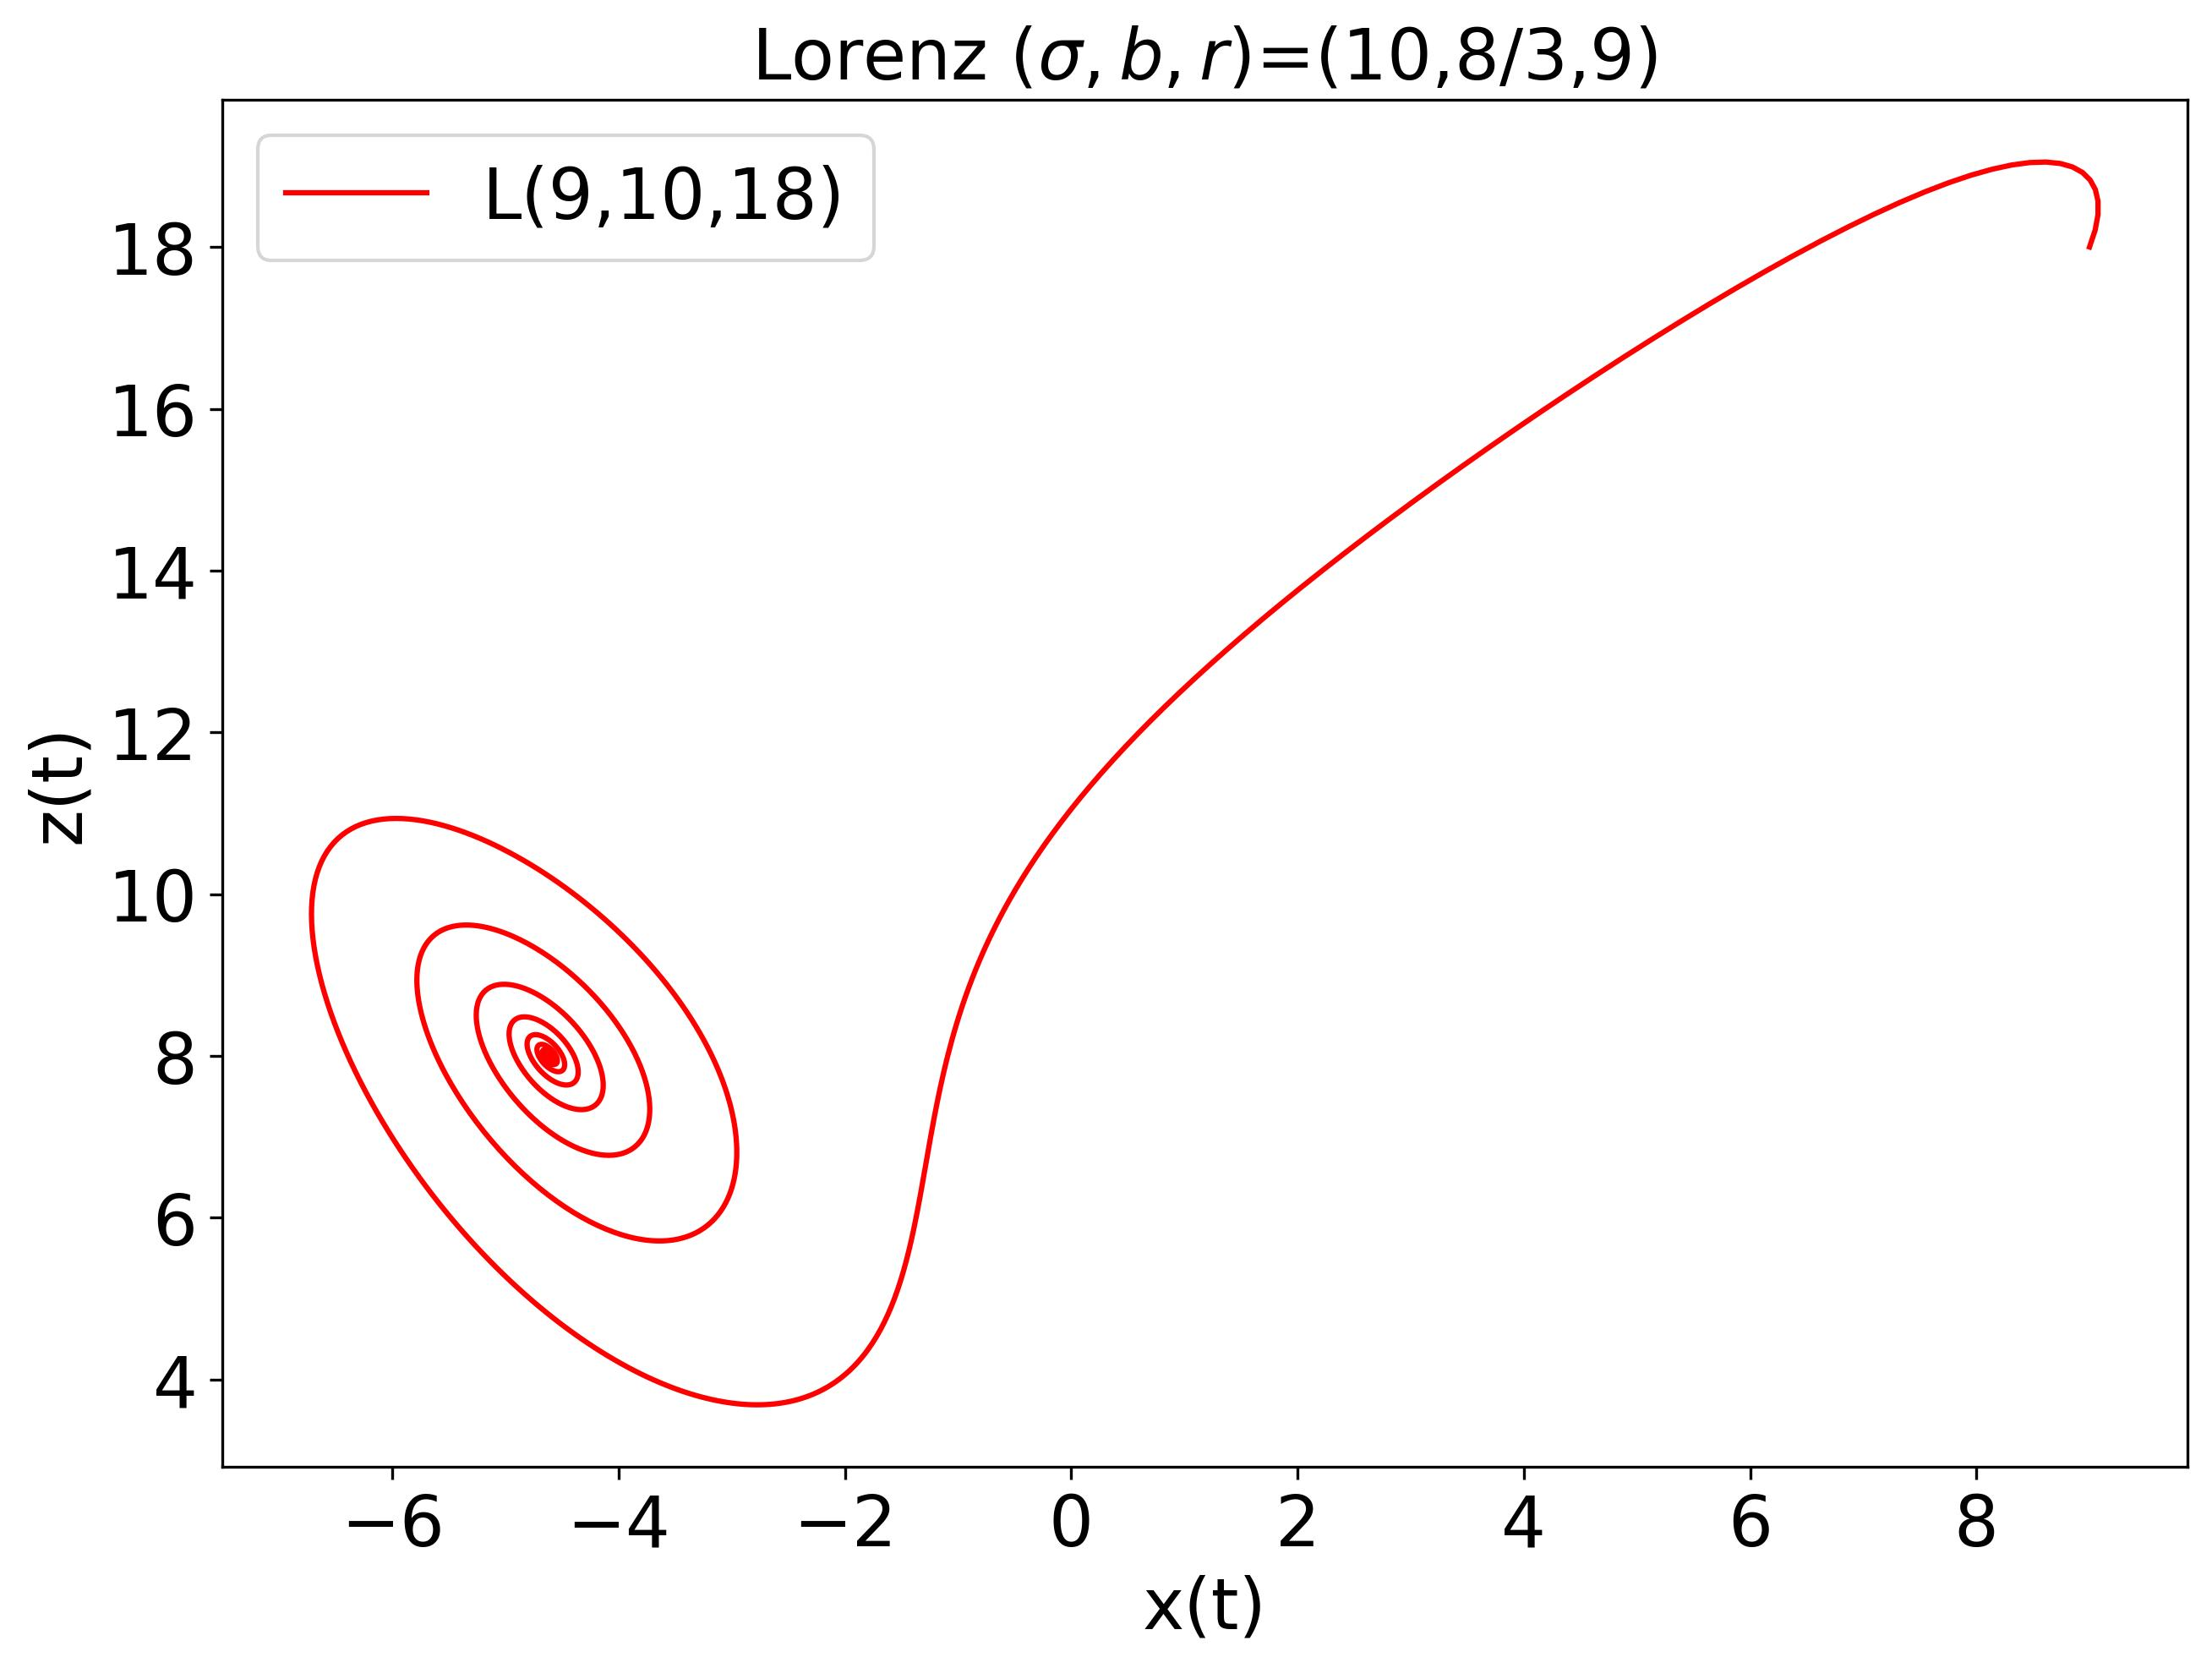
\includegraphics[width=\textwidth]{../xz_B.jpg}
        \caption{Set B}
        \label{fig:xz_b}
    \end{subfigure}
    \caption{\textit{Lorenz system trajectories with the same initial conditions and two different sets of parameters $(\sigma, b, r)$.}}
    \label{fig:xz}
\end{figure}

The trajectory in Figure \ref{fig:xz} with set A shows chaotic behavior, whereas the trajectory with set B is stable. In case B, the set of parameters describes a system where, given the same initial condition as in case A, the trajectory converges to a single point.

\begin{figure}[htbp]
    \centering
    \begin{subfigure}[t]{0.49\textwidth}
        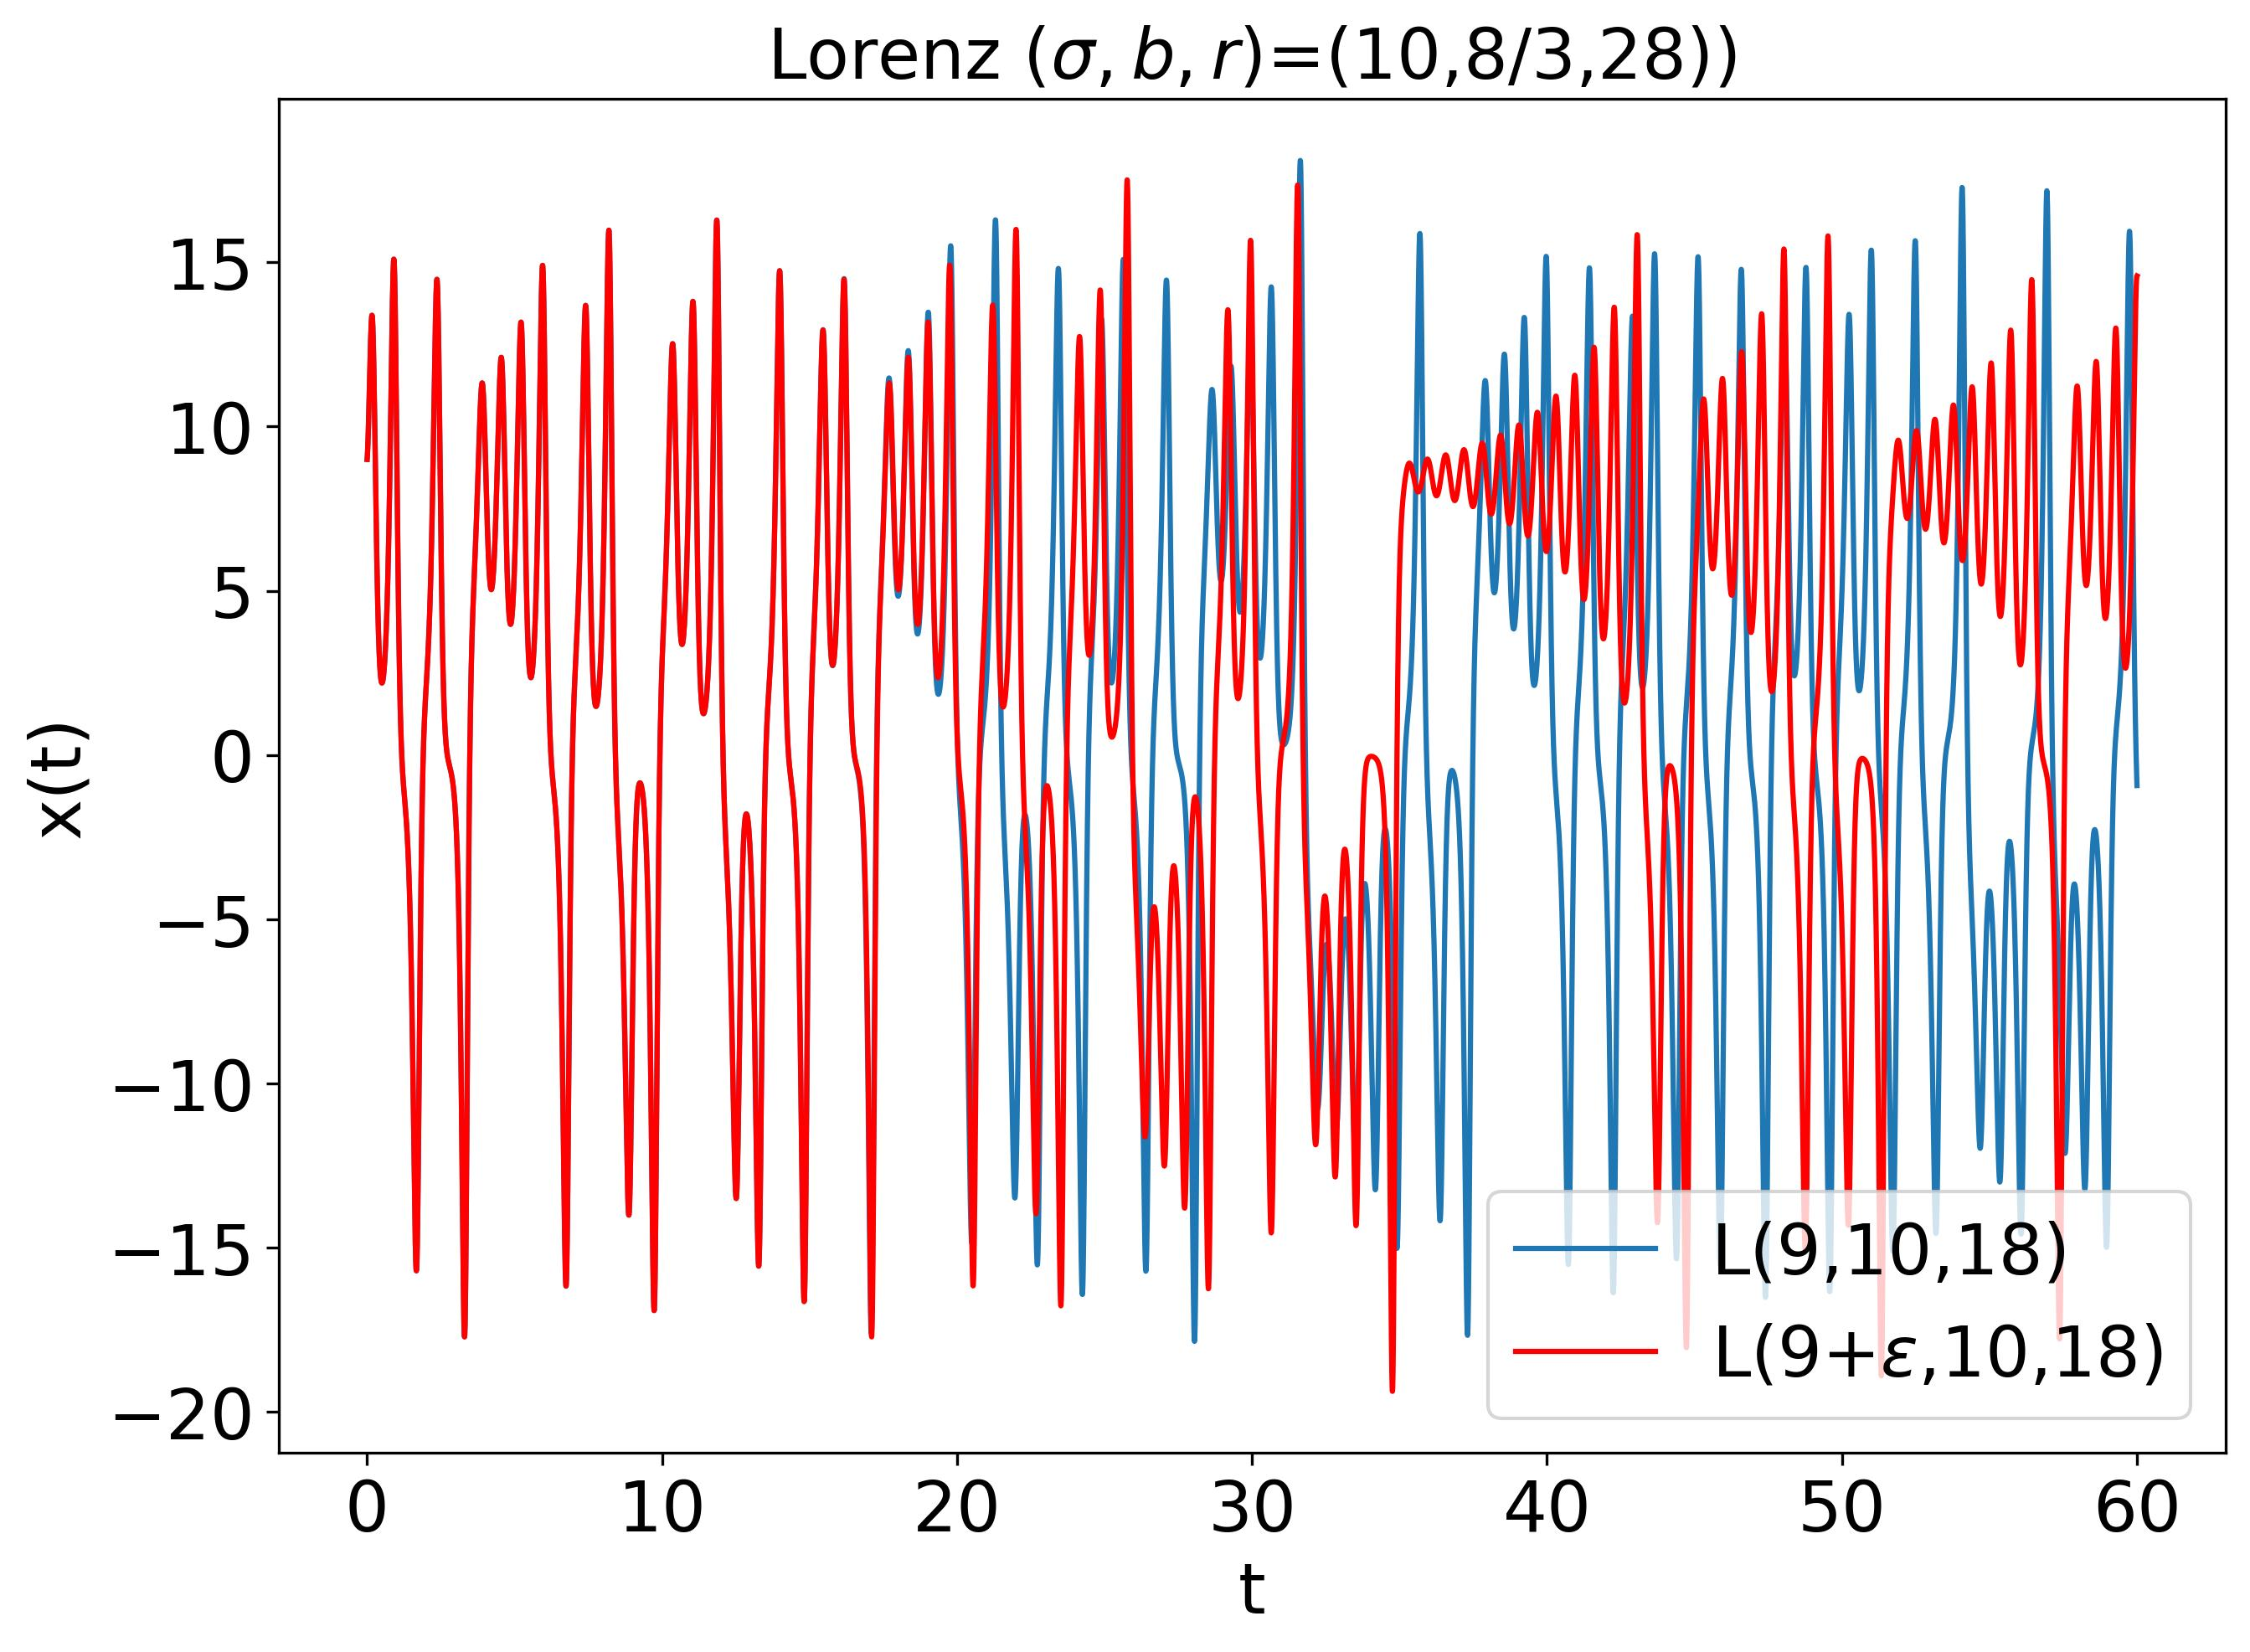
\includegraphics[width=\textwidth]{../pert_x(t)_A.jpg}
        \caption{Set A}
        \label{fig:pert_a}
    \end{subfigure}
    \hfill
    \begin{subfigure}[t]{0.49\textwidth}
        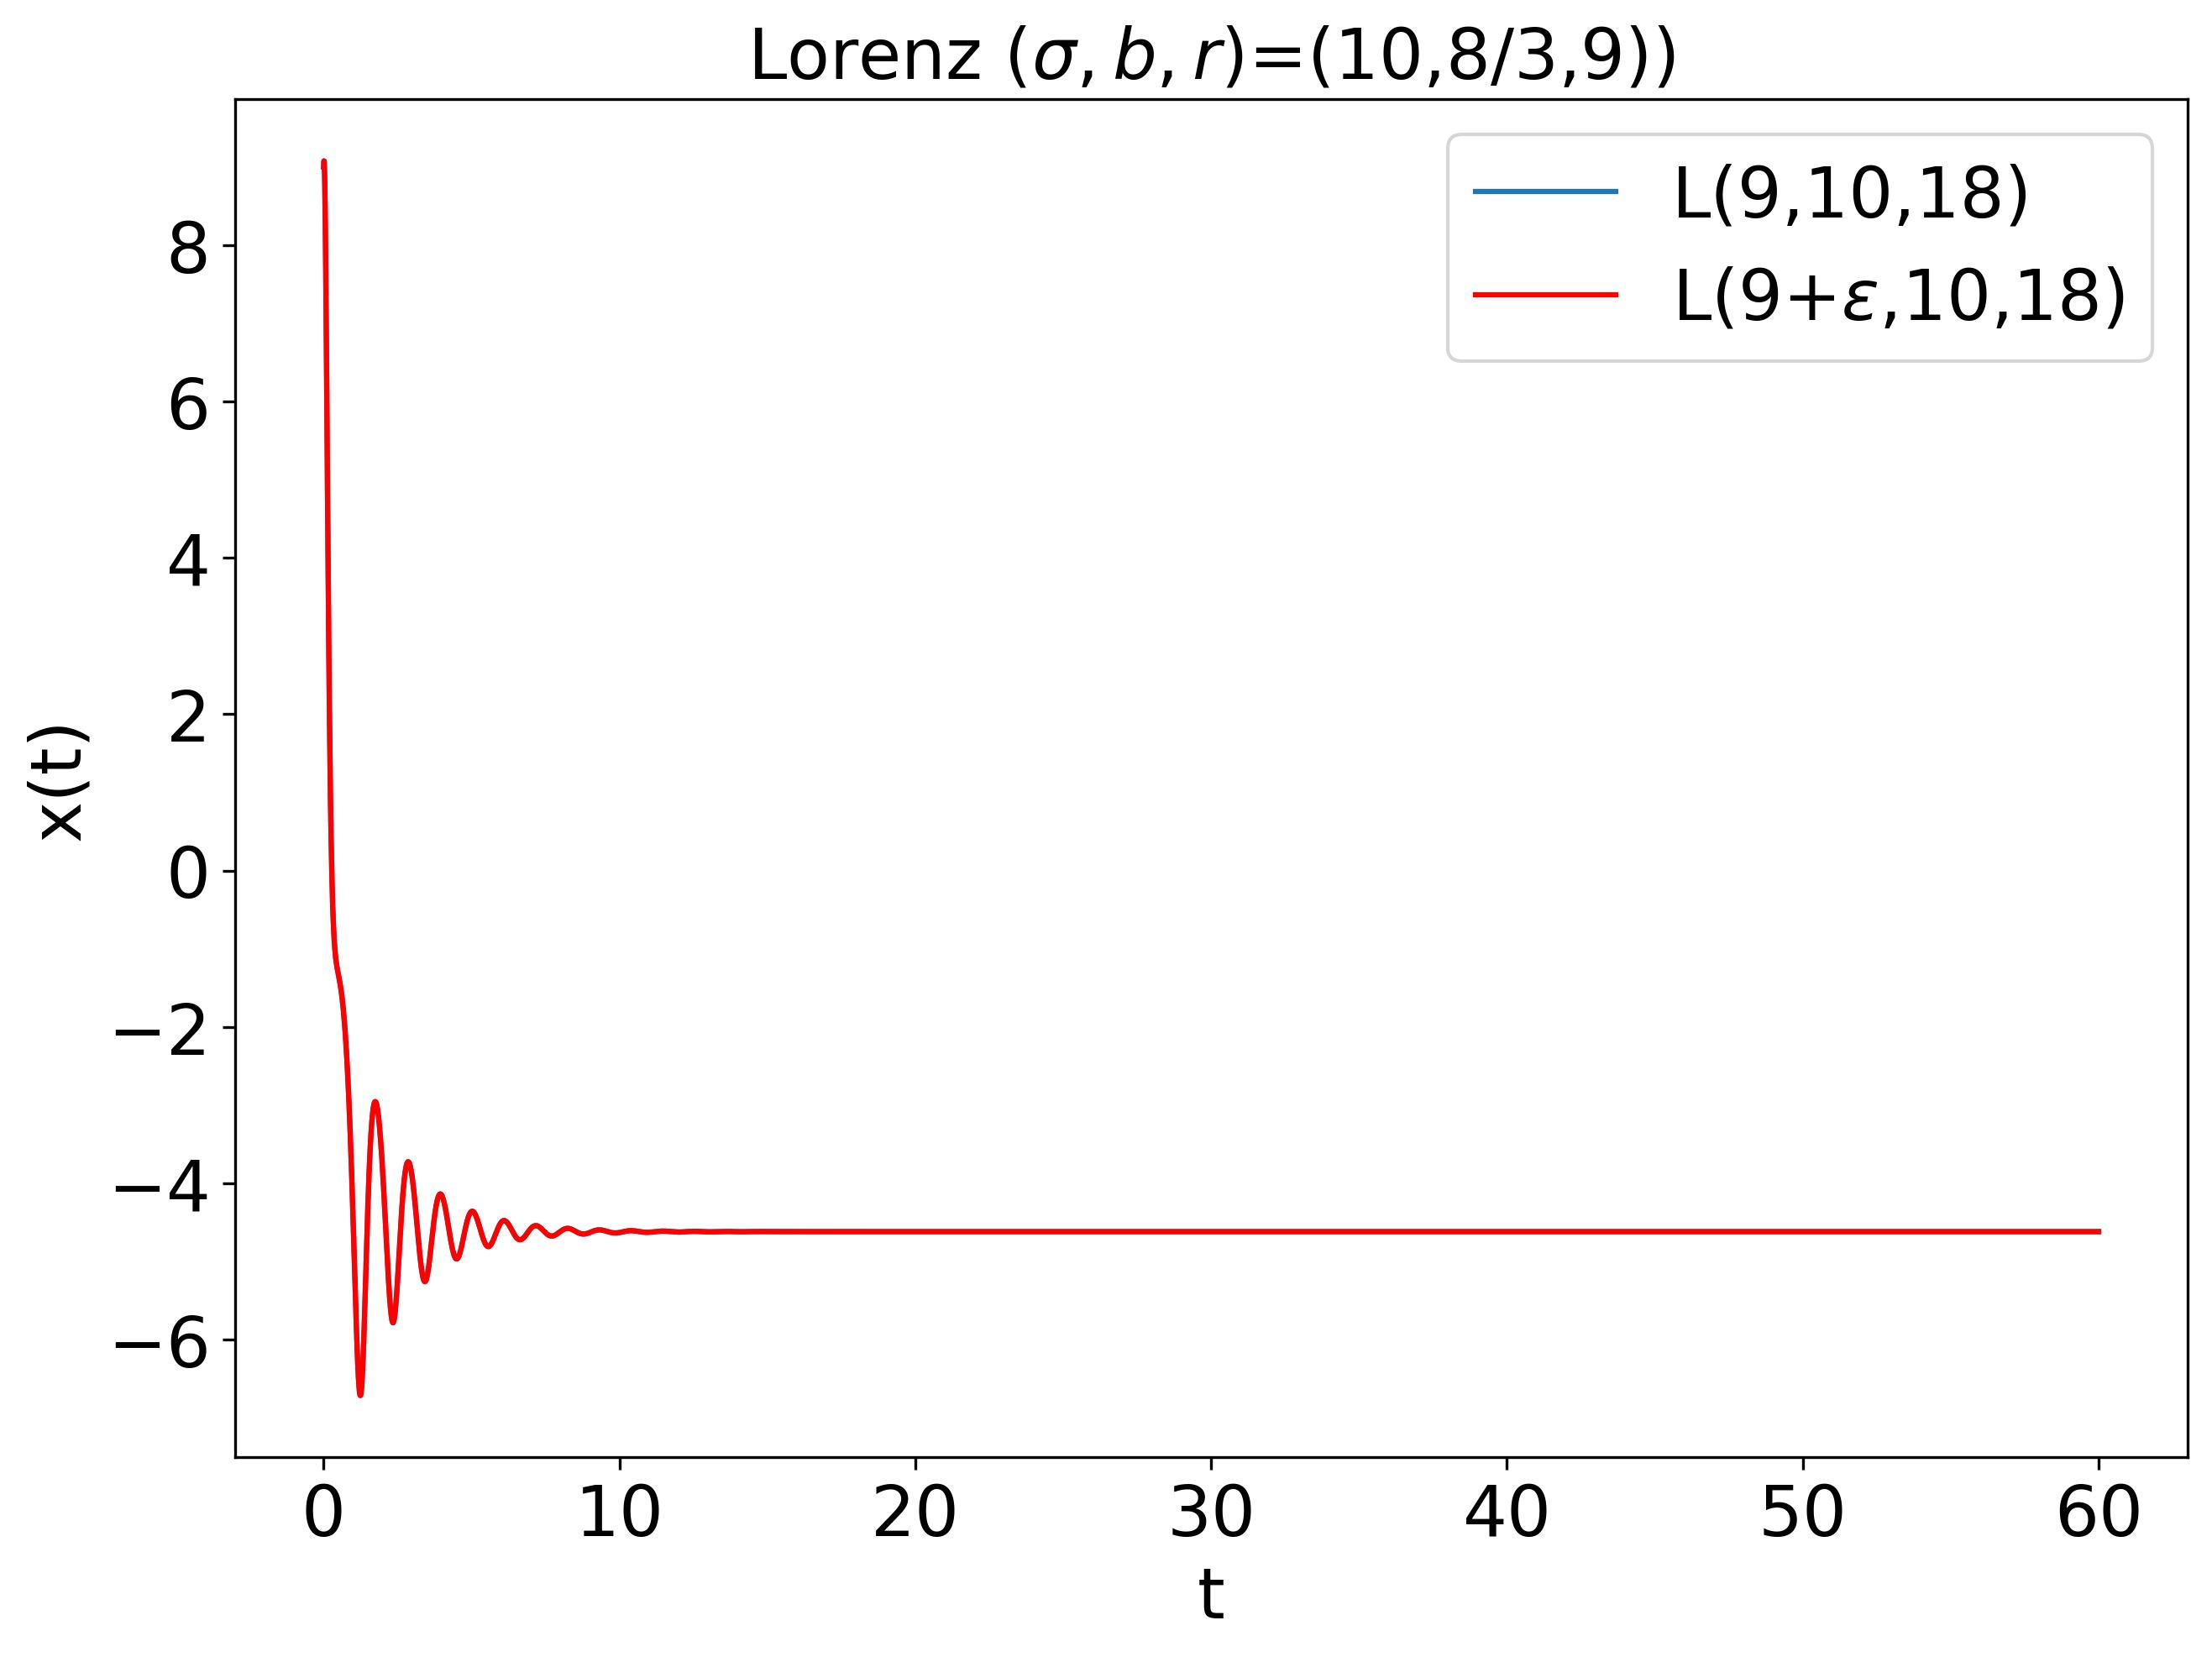
\includegraphics[width=\textwidth]{../pert_x(t)_B.jpg}
        \caption{Set B}
        \label{fig:pert_b}
    \end{subfigure}
    \caption{\textit{Comparison between the trajectory with an initial condition perturbed by $\epsilon=1\cdot10^{-7}$ and the unperturbed one, for both sets of parameters.}}
    \label{fig:pert_diff}
\end{figure}

The simulation is repeated with a perturbed initial condition 
$(9+\epsilon,10,18)$, Figure \ref{fig:pert_diff}. Comparing the results with the unperturbed case highlights a key point: in set A, the trajectories are initially close but end with significantly different x-coordinates, this distance is comparable to the size of the system's attractor. In set B, the two trajectories remain almost identical.

\begin{figure}[h]
    \centering
    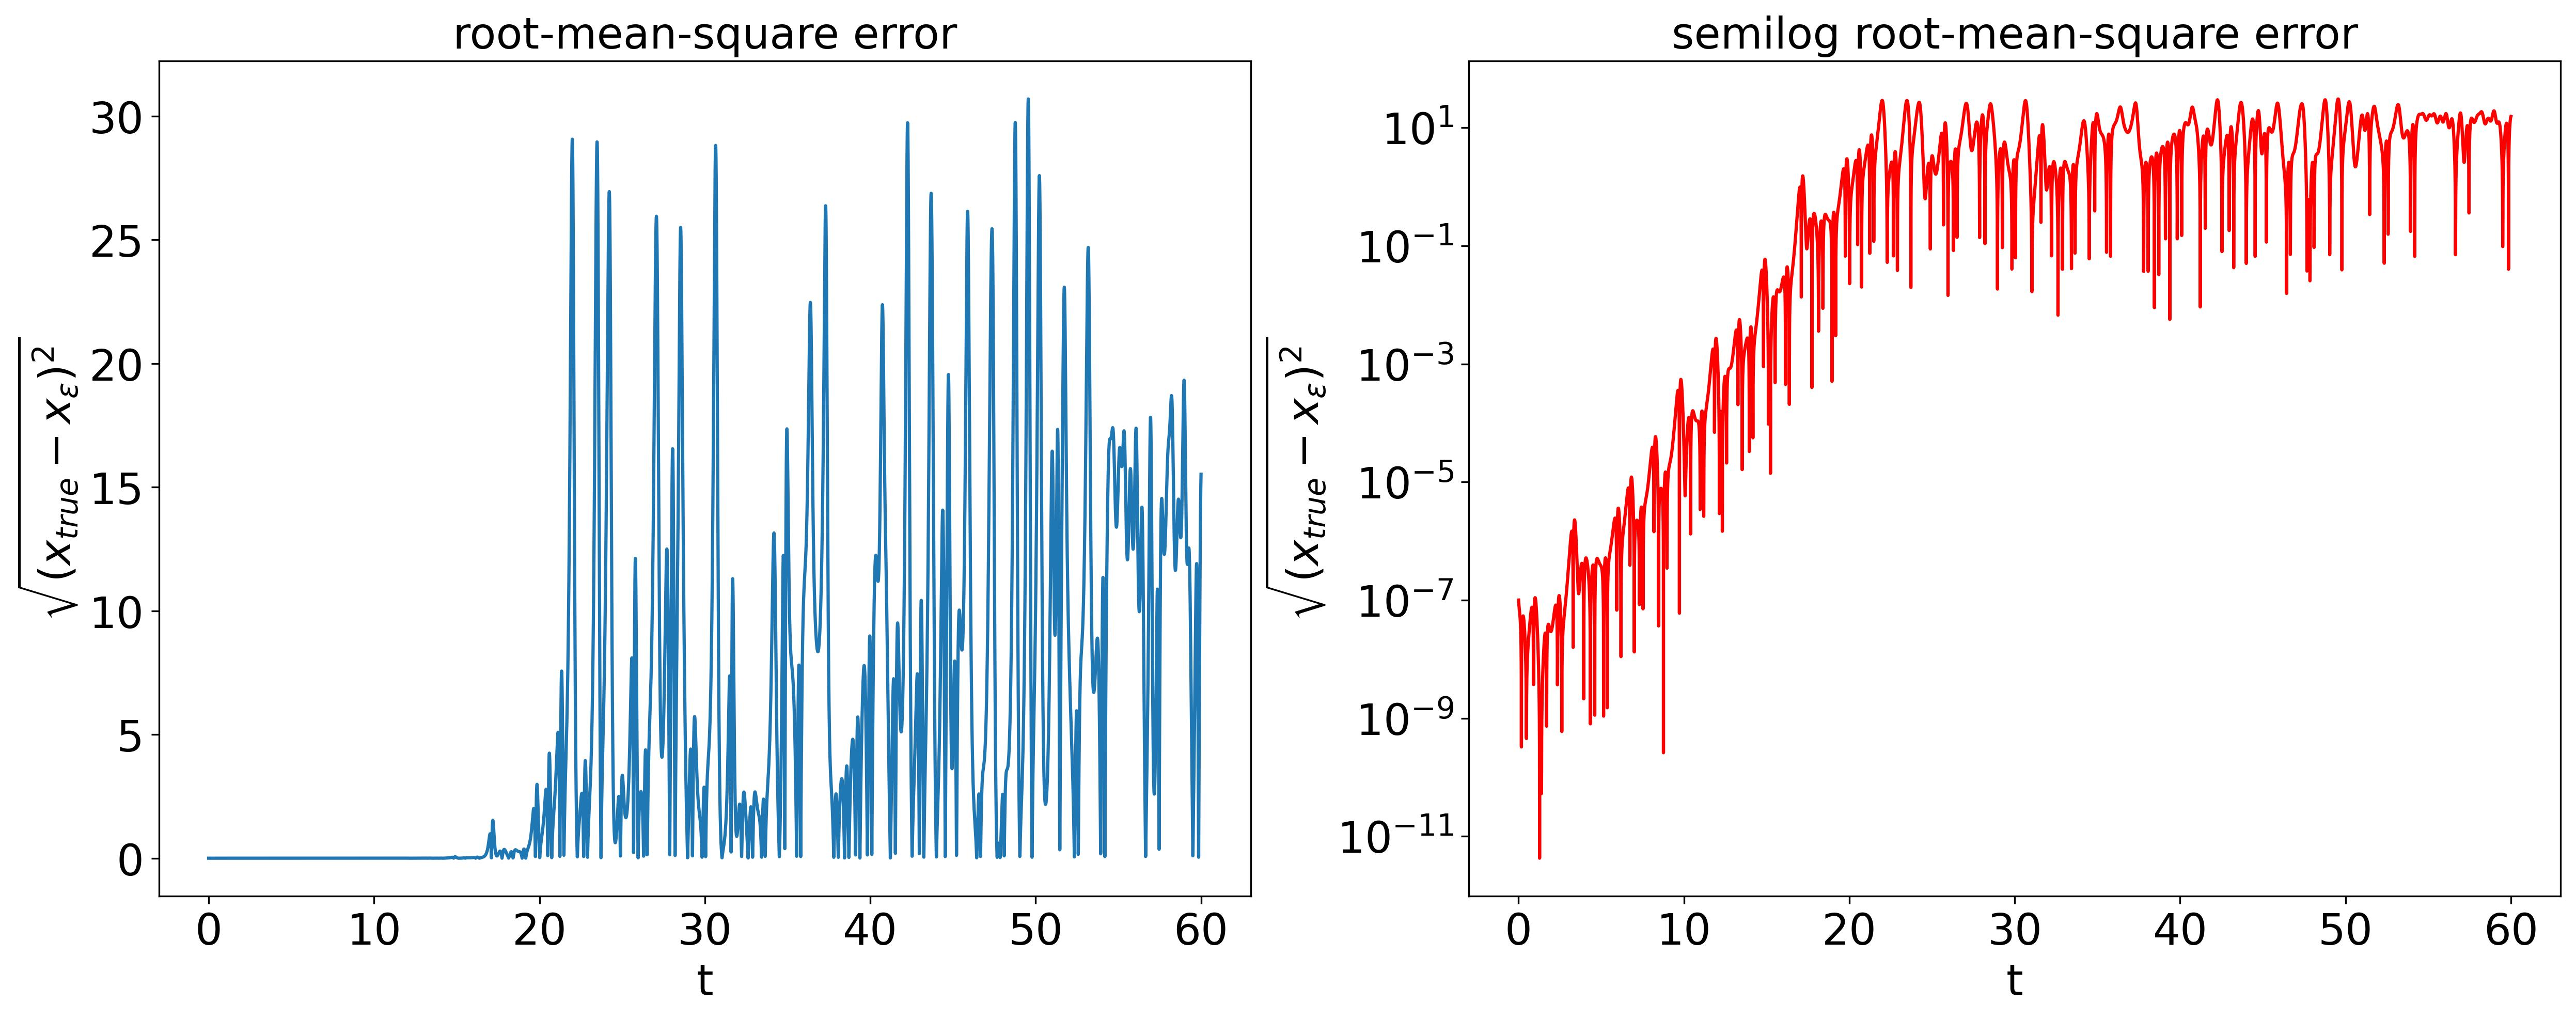
\includegraphics[width=\linewidth]{../rmse_A.jpg}
    \caption{\textit{Root-mean-square error versus time with set A. $x_{true}$ integrated with $L_0(9,10,18)$ and $x_\epsilon$ with $L_0(9+\epsilon,10,18)$.}}
    \label{fig:rmse_A}
\end{figure}
The difference between the perturbed and unperturbed trajectories confirms the statements above, Figure \ref{fig:rmse_A}. The x-values are similar at the beginning of the simulation but then diverge significantly. A notable feature is that the RMSE increases almost linearly on a semilog scale and, after a certain time step, saturates at a value comparable to the total range of the system's x-coordinates, the size of the attractor.
\newpage
\section{Ensemble of initial condition}

\begin{figure}[h]
    \centering
    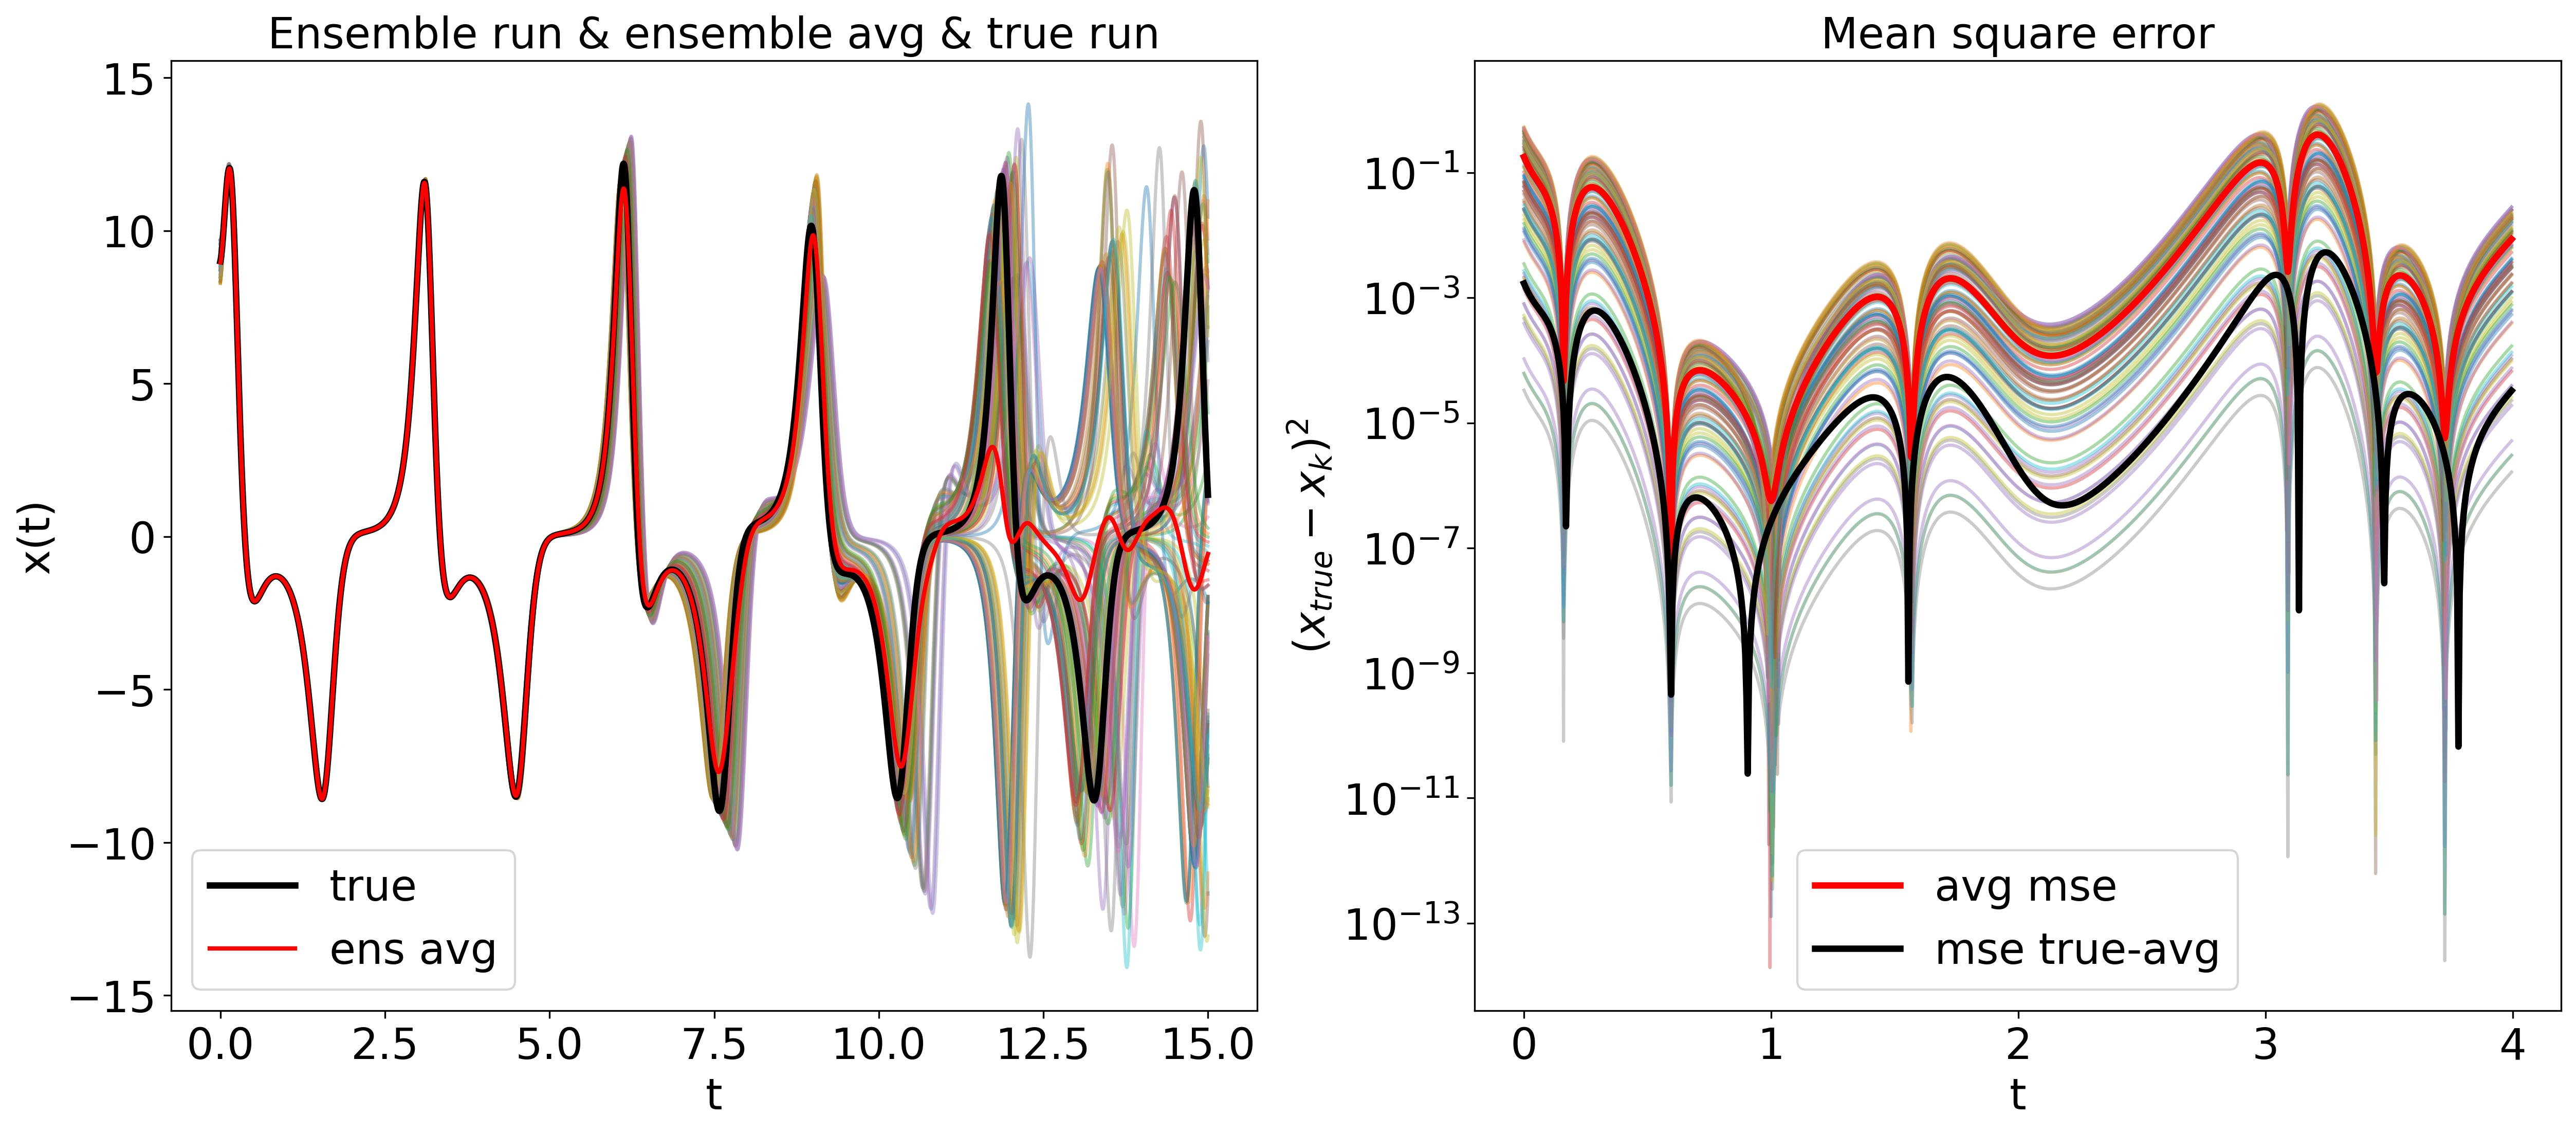
\includegraphics[width=\linewidth]{../ens_A.jpg}
    \caption{\textit{On the left, the trajectory along x of the hundred members of the ensemble (colored lines), their average (red line), and the trajectory with the unperturbated initial condition (black line). On the right, the comparison between the average mean square error $\langle R^2\rangle$ (red line) and the RMSE of the average $\langle x\rangle$ (black line), up tp $t=4$. The colored lines represent the RMSE of the individual members.}}
    \label{fig:ens_A}
\end{figure}

One hundred runs are performed with perturbed initial conditions $L(9+\epsilon,10,18)$, with $\epsilon$ uniformly extracted from -0.75 to 0.75 and set of parameters A. In Figure \ref{fig:ens_A}, on the left, the graph shows the trajectories over time of the ensemble members, with the average of the members in red and the run without perturbation in black. It can be seen that after a certain time, the ensemble members explore almost all available regions and their average therefore approaches zero.
In the graph on the right, the red line is the average of the mean square errors of the individual members (colored lines),
\begin{equation}
    \langle R^2\rangle = \frac{1}{N} \sum_{k=1}^{N} (x_{true} - x_k)^2
\end{equation}
while the black one is the mean square error of the ensemble average $(x_{true} - \langle x \rangle)^2$.
The average MSE is always greater than the MSE of the ensemble average by at least two orders of magnitude, this implies that the ensemble average follows the true trend very closely. However, the average of the members no longer represents the true value when we move far away from the initial moment.

\newpage
\section{Response to a forcing}
A positive forcing is inserted into the Lorenz system in the derivative of y, Figure \ref{fig:forcing}. It is integrated with the set of parameters A and 50 different initial conditions: x and y extracted uniformly between -20 and 20 and z between 0 and 30. The integration time extends up to 200, is divided into intervals of 5000 time steps, and in each one the probability of having $x < 0$ is calculated.

\begin{figure}[h]
    \centering
    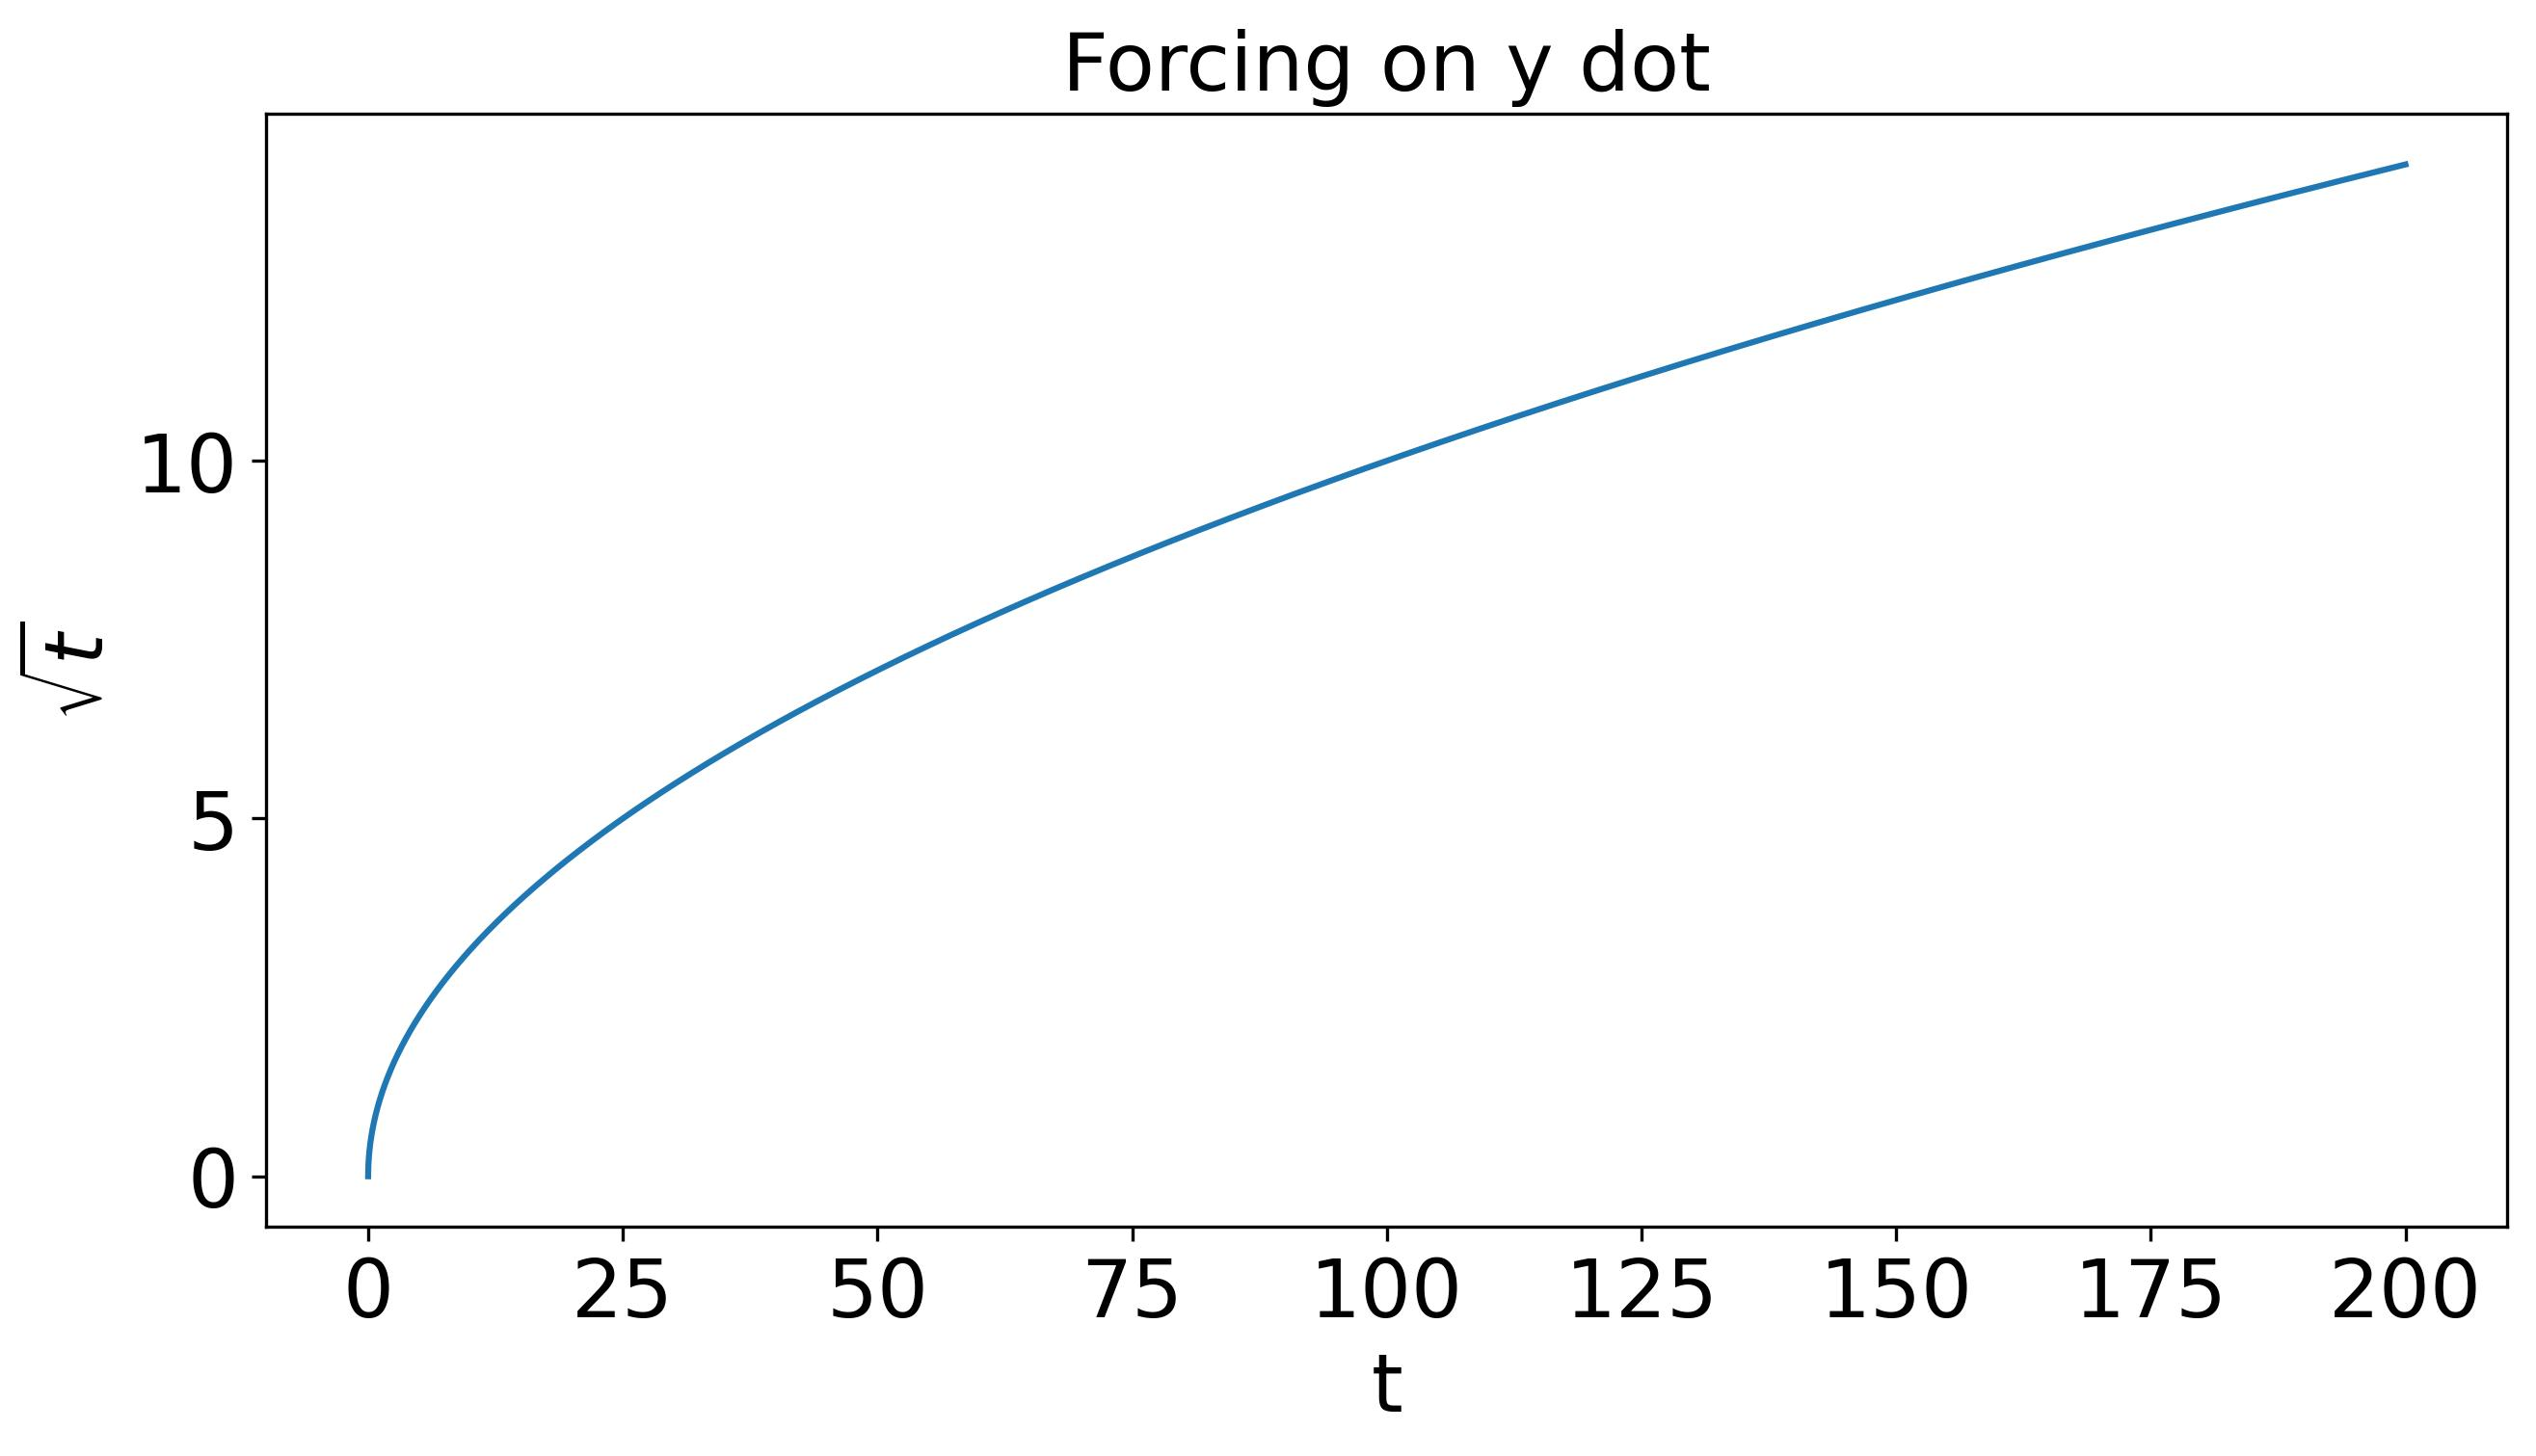
\includegraphics[width=0.5\linewidth]{../forcing_A.jpg}
    \caption{\textit{The forcing applied to the system.}}
    \label{fig:forcing}
\end{figure}

In Figure \ref{fig:prob}, the colored lines represent the probability of having negative x for each member of the ensemble as a function of time, while the black line is the average for each tau across all members. The 50 horizontal blue lines are the overall average probabilities for each member.\\
It can be seen that without forcing, the probability of having negative x values is around 50\% considering all members, and remains constant over time (black line). The overall probabilities of the individual members are distributed symmetrically around 50\% (blue lines). This symmetry is broken by introducing the forcing, with the individual average probabilities falling below 50\% and becoming more tightly clustered. The probability of having negative x values decreases over time to 40\%, despite the members maintaining a wide variability.

\begin{figure}[h]
    %\vspace{-6in}
    \centering
    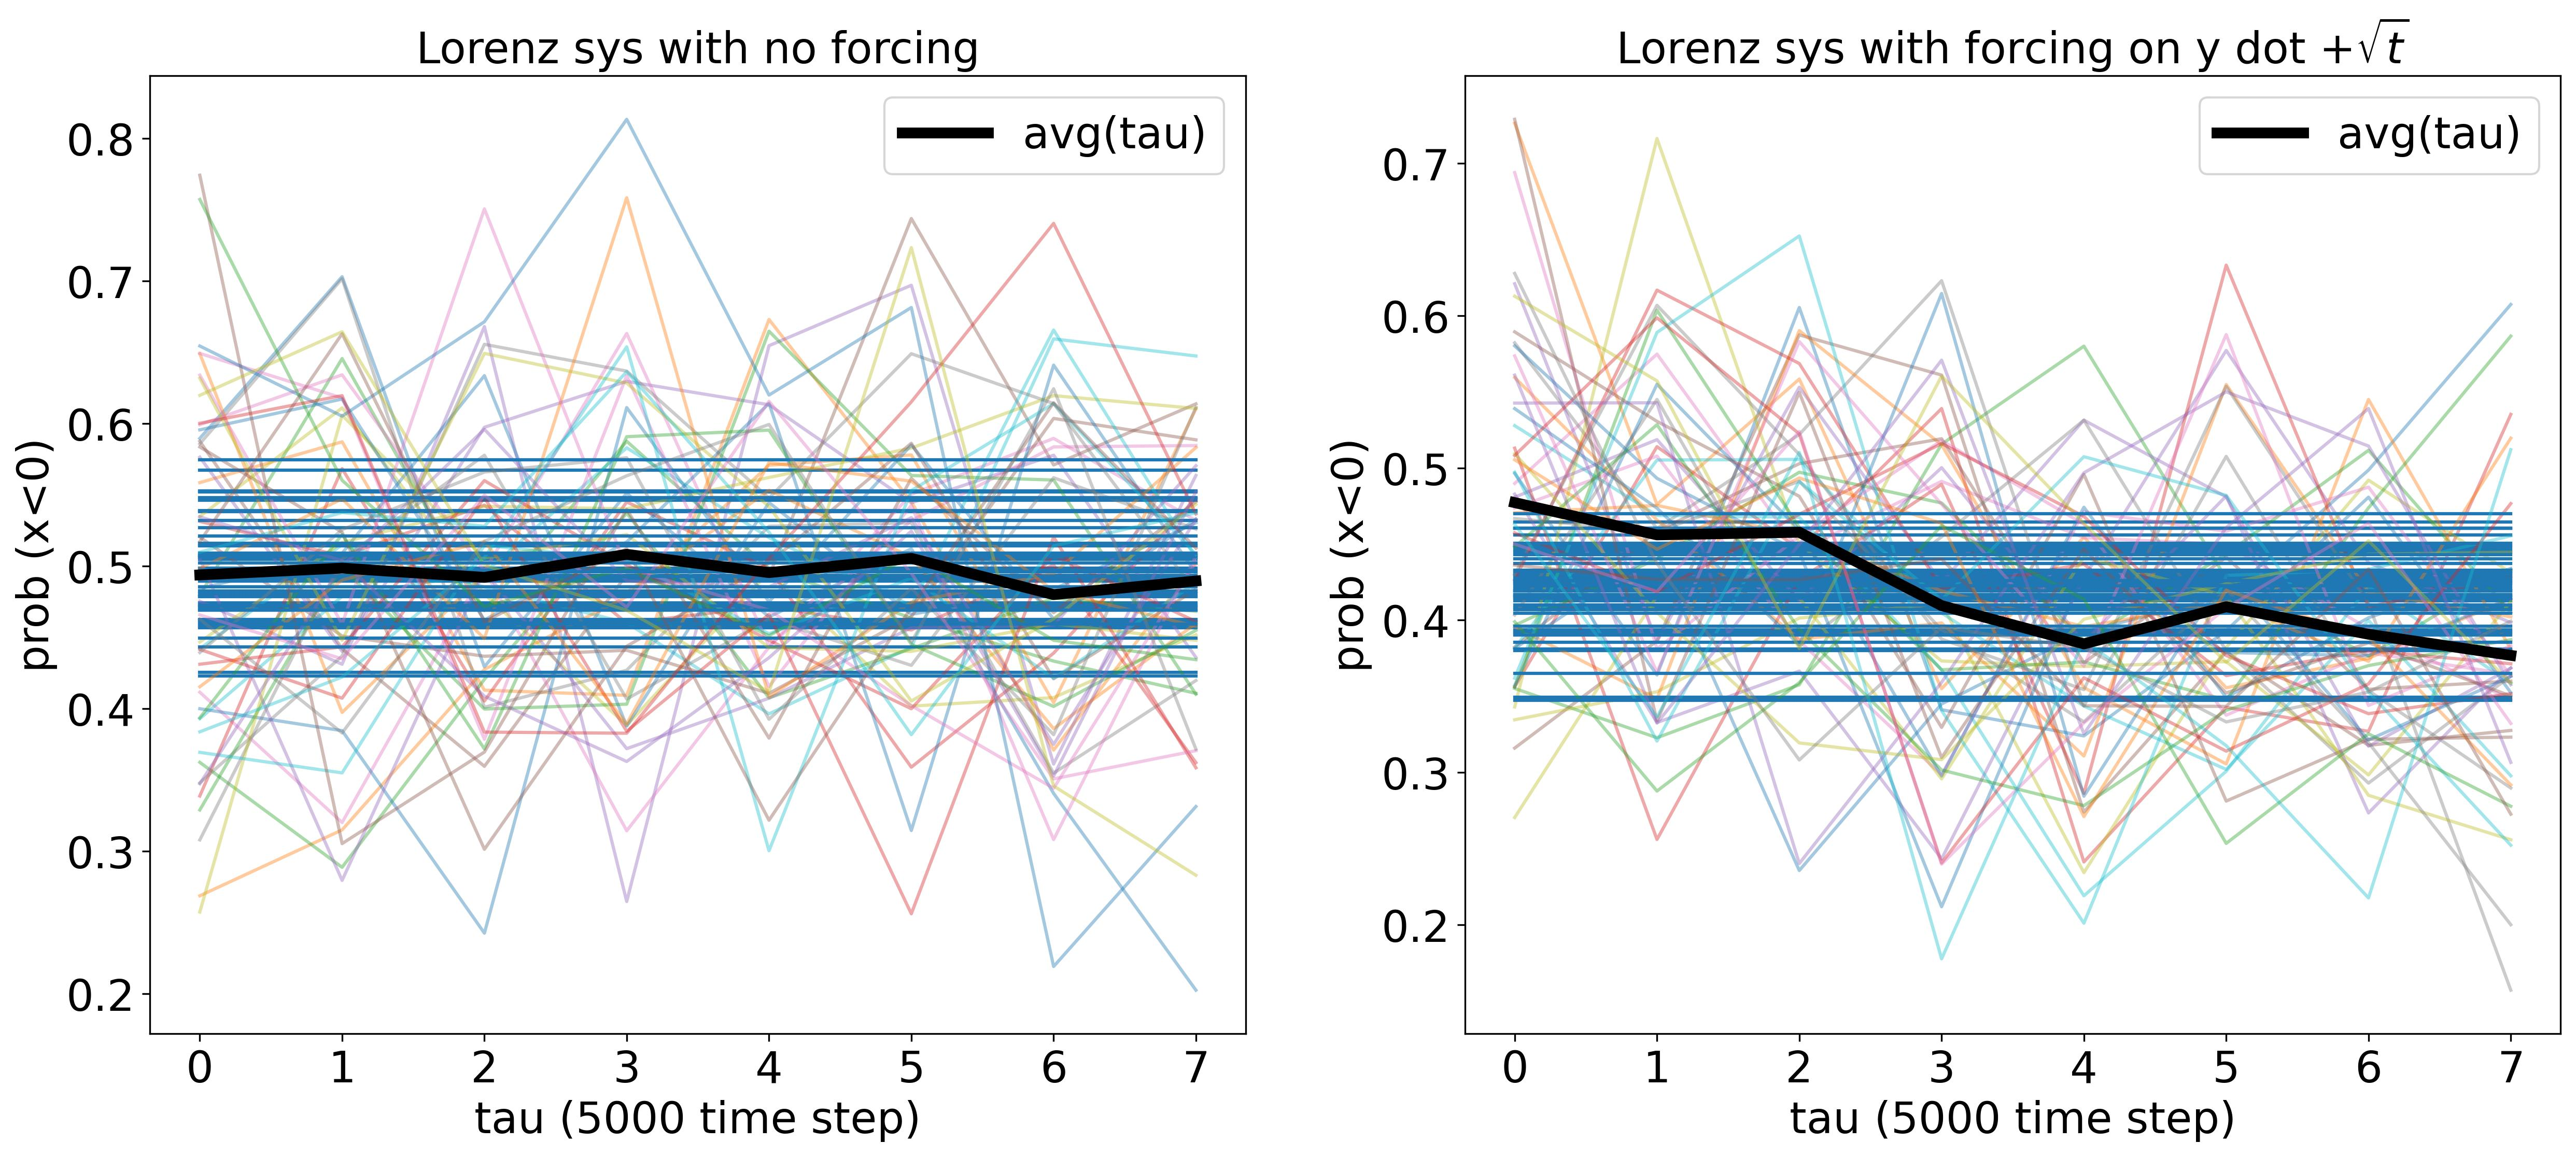
\includegraphics[width=\linewidth]{../ens_forcing_A.jpg}
    \caption{\textit{Comparison between the probability of $x<0$ in the absence of forcing, on the left, and with forcing on the right. The colored lines represent $P_k(\tau)$, the blue lines $P_k$ and the black line the average over all memebers $P(\tau)$.}}
    \label{fig:prob}
\end{figure}

\newpage
\section{Conclusions}
A simplified system such as the one proposed by Lorenz makes it easy to highlight how a chaotic system is highly dependent on initial conditions or not, based on the physical parameters used. It is clear that using an ensemble is useful for reducing the effects of chaos, but care must be taken to determine how reliable they can be considered to be over time. Finally, we observe how the system reacts to a forcing: chaos is maintained and only through averaging operations is it possible to evaluate the effect that the forcing has on the system.

\begin{comment}
\begin{figure}[htbp]
    \centering
    \begin{subfigure}[t]{0.49\textwidth}
        \includegraphics[width=\textwidth]{}
        %\caption{Didascalia 1}
        %\label{fig:img1}
    \end{subfigure}
    \hfill
    \begin{subfigure}[t]{0.49\textwidth}
        \includegraphics[width=\textwidth]{}
        %\caption{Didascalia 3}
        %\label{fig:img3}
    \end{subfigure}
    \hfill
    \begin{subfigure}[t]{0.49\textwidth}
        \includegraphics[width=\textwidth]{}
        %\caption{Didascalia 3}
        %\label{fig:img3}
    \end{subfigure}
    \hfill
    \begin{subfigure}[t]{0.49\textwidth}
        \includegraphics[width=\textwidth]{}
        %\caption{Didascalia 3}
        %\label{fig:img3}
    \end{subfigure}
    \caption{\textit{}}
    \label{fig:}
\end{figure}
\end{comment}

\end{document}
